\textbf{Принадлежности:} установка для определения отношения молярных теплоемкостей газа адиабатическим методом.

\begin{center}
    \textbf{Оборудование.}
\end{center}

Для проведения опыта служит прибор (рис. \ref{fig:установка 3.}), состоящий из большой стеклянной бутыли A, в горловину которой вставлена герметичная пробка. Через пробку проходит латунная трубка, имеющая два отвода: один a соединен с насосом, служащим для накачивания воздуха в сосуд, другой c – с манометром M. Сверху латунная трубка плотно закрывается резиновой пробкой в.

\begin{figure}[!h]
    \centering
    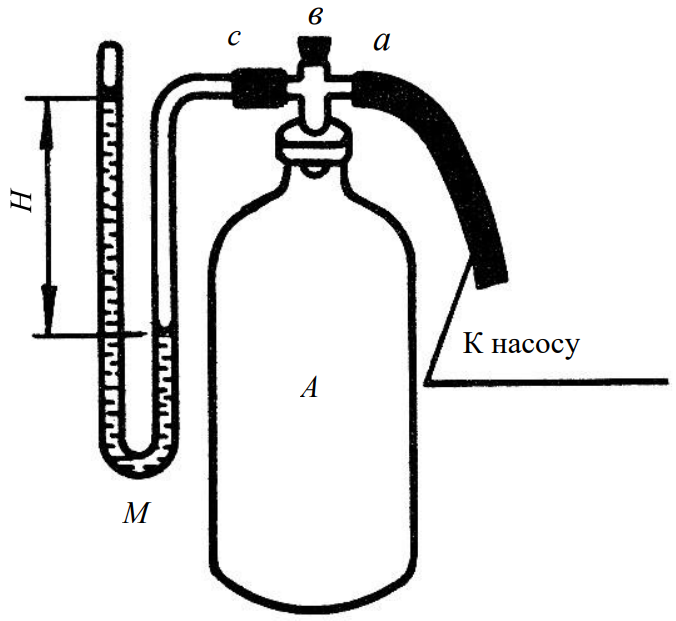
\includegraphics[width = 0.3\textwidth]{image/image3.png}
    
    \caption{Установка для Определения отношения молярных теплоемкостей газа адиабатическим методом.}
    
    \label{fig:установка 3.}
\end{figure}

Отношение количества теплоты $dQ$, сообщенного системе (телу), к соответствующему повышению температуры $dT$ называют теплоёмкостью:

\begin{equation}
    C_\text{тела} = \frac{d Q}{d T}
    \label{eq:formula_1}
\end{equation}

Наиболее распространенным является определение теплоёмкости как количества теплоты, которое необходимо затратить для изменения температуры тела на один градус.

Теплоёмкость единицы массы вещества называют удельной: 

\begin{equation*}
c = \frac{1}{m} \cdot \frac{d Q}{d T} [\frac{\text{Дж}}{\text{кг} \cdot \text{К}}]
\end{equation*}

Теплоёмкость моля вещества называют молярной:

\begin{equation}
c = \frac{1}{\nu} \cdot \frac{d Q}{d T} [\frac{\text{Дж}}{\text{моль} \cdot \text{К}}]
    \label{eq:formula_2}
\end{equation}

Иногда употребляется внесистемная единица теплоѐмкости: $\frac{\text{кал}}{\text{моль*град}}$. Калория "--- внесистемная единица измерения количества теплоты (1 кал = 4,187 Дж).

Удельная и молярная теплоѐмкости связаны соотношением.

$c = \frac{C}{M}$, где M "--- молярная масса.

Приведенное выше определение теплоёмкости (\ref{eq:formula_1}) не является достаточным, так как количество теплоты $dQ$, сообщаемое телу, зависит от характера процесса, в результате которого система перешла в новое состояние. Другими словами, необходимо еще указать условия, при которых производится передача количества тепла. Эта неопределенность  обусловлена тем, что количество теплоты не является функцией состояния тела в отличие, например, от внутренней энергии

В связи с отмеченной неоднозначностью возможны различные определения теплоёмкости. Так, для термодинамической системы, состояние которой определяется: давлением ($p$), объёмом ($V$) и температурой ($T$), различают теплоёмкости при постоянном объеме $CV$ и постоянном давлении $Cp$. Эти теплоёмкости характеризуются количеством тепла, сообщаемым системе в условиях, когда остается неизменным либо объем, либо давление.

Согласно первому закону термодинамики, выражающему закон сохранения энергии в области тепловых явлений, количество теплоты $dQ$, сообщаемое системе, затрачивается на увеличение внутренней энергии системы $dU$ и на работу $dA$, которую система совершает над внешней средой:

\begin{equation}
    d Q = d U + d A
    \label{eq:formula_3}
\end{equation}

(Более строго, это соотношение записывается в виде $\delta Q = dU + \delta A$, чтобы подчеркнуть то обстоятельство, что $dU$ является полным дифференциалом, поскольку среди величин $Q$, $U$ и $A$ только $U$ является функцией состояния системы.)
	Работа $dA$ в случае отсутствия магнитных и электрических явлений сопровождается исключительно расширением системы, которая находится под действием внешнего давления $p$, и в этом случае $dA = p \cdot dV$ ($dV > 0$). Тогда

\begin{equation}
    d Q = d U + p \cdot d V
    \label{eq:formula_4}
\end{equation}

Если нагревание происходит при постоянном объеме $V = const$ ($dV = 0$), то все тепло тратится на увеличение внутренней энергии:

$d Q = d U$

Тогда из определения молярной теплоёмкости (\ref{eq:formula_2}):


\begin{equation*}
    C_V = \left (\frac{d Q}{d T} \right)_V = \left (\frac{d U_0}{d T} \right )_V
\end{equation*}

где $U_0$ "--- внутренняя энергия одного моля газа. Отсюда для идеального газа можно записать.


\begin{equation}
    C_V = \frac{d U_0}{d T}
    \label{eq:formula_5}
\end{equation}

так как внутренняя энергия является только функцией температуры $U(T)$.

Для изобарического процесса ($p = const$) из (\ref{eq:formula_4}) и (\ref{eq:formula_5}) следует:

\begin{equation}
    C_p = \left (\frac{d Q}{d T} \right )_p = \frac{d U_0}{d T} + p \left (\frac{d V}{d T} \right )_p = C_V + p \left (\frac{d V}{d T} \right)
    \label{eq:formula_6}
\end{equation}

В соответствии с уравнением состояния идеального газа (для одного моля газа $\nu = 1$)

\begin{equation}
    p V = R T
    \label{eq:formula_7}
\end{equation}

При $p = const$

\begin{equation*}
    \left (\frac{d V}{d T} \right )_p = \frac{R}{p}
\end{equation*}

тогда

\begin{equation}
    C_p = C_V + R
    \label{eq:formula_8}
\end{equation}

Теплоёмкость $Cр$ всегда больше теплоёмкости $CV$. Это связано с работой, совершаемой газом при расширении ($p = const$).

При описании некоторых физических процессов приходится иметь дело с отношением теплоемкостей

\begin{equation}
    \gamma = \frac{C_p}{C_V}
    \label{eq:formula_9}
\end{equation}

Одним их таких процессов, играющих важную роль при изучении тепловых явлений, является адиабатический процесс. Для этого процесса характерна теплоизолированность системы от внешней среды, т. е. процесс протекает без теплообмена с внешней средой. Значит, работа, совершаемая системой в этом случае, производится за счет изменения ее внутренней энергии. Из первого закона термодинамики (\ref{eq:formula_3}) для адиабатического процесса ($dQ = 0$) имеем 

\begin{equation}
    d u + p \cdot d v = 0
    \label{eq:formula_10}
\end{equation}

В случае идеального газа (\ref{eq:formula_5}) для одного моля $dU_0 = CV \cdot dT$. Тогда с учетом этого выражение (\ref{eq:formula_10}) примет вид

\begin{equation}
    C_V d T + p \cdot dV = 0
    \label{eq:formula_11}
\end{equation}

Дифференцируя уравнение (\ref{eq:formula_7}), получим:

\begin{equation*}
    p d V + V d p = R d T
\end{equation*}

и выразим из полученного выражения $dT$:

\begin{equation}
    d T = \frac{1}{R} \left (p d V + V d p \right )
    \label{eq:formula_12}
\end{equation}

Подставим (\ref{eq:formula_12}) в (\ref{eq:formula_11}):

\begin{equation*}
    \frac{c_v}{r} \left (p d v + v d p \right ) + p d v = 0
\end{equation*}

Преобразования последнего выражения с учётом (\ref{eq:formula_8}) и (\ref{eq:formula_9}) дают:

\begin{equation*}
    \frac{C_V + R}{R} p d V + \frac{C_V}{R} V d p = 0
\end{equation*}

\begin{equation*}
    \frac{C_p}{C_V} \cdot \frac{d V}{V} + \frac{d p}{p} = 0
\end{equation*}

\begin{equation}
    \gamma \frac{d V}{V} + \frac{d p}{p} = 0
    \label{eq:formula_13}
\end{equation}

Интегрирование (\ref{eq:formula_13}) даёт:

\begin{equation*}
    \gamma \ln(V) + \ln(p) = const
\end{equation*}

откуда следует, что

\begin{equation}
    p V^ \gamma = const
    \label{eq:formula_14}
\end{equation}

С учётом (\ref{eq:formula_7}) уравнение (\ref{eq:formula_14}) примет вид

\begin{equation}
    T \cdot V^(\gamma - 1) = const
    \label{eq:formula_15}
\end{equation}

Соотношения (\ref{eq:formula_14}) и (\ref{eq:formula_15}) называют уравнениями Пуассона.

Молекулярно-кинетическая теория, рассматривая газ как совокупность свободно движущихся частиц, подчиняющихся законам классической механики, позволяет удовлетворительно объяснить некоторые основные свойства реальных газов. В частности, она дает возможность оценить порядок величин термодинамических характеристик $Cp$, $CV$ и $\gamma$.

Согласно представлениям кинетической теории, молекулы идеального газа не взаимодействуют между собой, внутренняя энергия такого газа не зависит от изменения объема и давления и является только функцией температуры. В силу полной беспорядочности движения считают, что в среднем на каждую степень свободы приходится энергия, равная $\frac{kT}{2}$ , где $k = 1,3807 \cdot 10^(–23) \frac{\text{Дж}}{\text{К}}$ "--- постоянная Больцмана.

Если рассматривать одноатомный газ, каждая частица которого представляется как точечная масса, совершающая поступательное движение и поэтому имеющая три степени свободы (положение ее в пространстве может быть определено тремя независимыми координатами), то средняя кинетическая энергия такой частицы равна $\frac{3}{2}kT$

Внутренняя энергия многоатомных газов складывается из кинетических энергий поступательного и вращательного движения молекул. Применяя и в этом случае положение о равном распределении энергии по степеням свободы, можно подсчитать среднюю кинетическую энергию $E_0$ многоатомной молекулы:

\begin{equation}
    E_0 = \frac{i}{2} k T
    \label{eq:formula_16}
\end{equation}

где i "--- число степеней свободы молекул. Молекулы двухатомного газа обладают тремя поступательными и двумя вращательными степенями свободы. Поэтому средняя кинетическая энергия двухатомной молекулы.

\begin{equation}
    E_0 = \frac{5}{2} k T
    \label{eq:formula_17}
\end{equation}

Внутреннюю энергию $U_0$ одного моля газа найдем, умножив (\ref{eq:formula_16}) на число молекул $NA$ в одном моле ($N_A = 6,022·10^23 моль^(-1)$ "--- число Авогадро):

\begin{equation}
    U_0 = \frac{i}{2} N_A k T = \frac{i}{2} R T
    \label{eq:formula_18}
\end{equation}

Молярную теплоёмкость газа при постоянном объеме получим, продифференцировав (\ref{eq:formula_18}) по температуре:

\begin{equation}
    C_p = \frac{d U_0}{d T} = \frac{i}{R}
    \label{eq:formula_19}
\end{equation}

Используя (\ref{eq:formula_7}) и (\ref{eq:formula_19}), выразим через число степеней свободы молекулы теплоёмкость $Cp$ и отношение теплоемкостей $\gamma$:

\begin{equation*}
    C_p = \frac{i}{2} R + R = \frac{i + 2}{2} R
\end{equation*}

\begin{equation*}
    \gamma = \frac{C_p}{C_V} = \frac{i + 2}{2}
\end{equation*}

В работе требуется найти отношение $\gamma$ теплоемкостей $Cp$ и $CV$ воздуха. Поскольку воздух состоит в основном из смеси двухатомных газов (водорода, кислорода, азота), каждая молекула которых имеет пять степеней свободы, то отношение молярных (или удельных в соответствии с соотношением $c = \frac{C}{M}$) теплоемкостей для воздуха будет $\gamma = 1.40$. Это довольно хорошо согласуется по порядку величины с экспериментальными данными, полученными для чистого воздуха, свободного от $CO_2$ и паров воды при нормальных условиях.

\begin{center}
    \textbf{Вывод рабочей формулы}
\end{center}











